\chapter{INTRODUCCIÓN}

	\vspace{10pt}

	Los avances actuales de la informática (2024) y la difusión global de la Internet han cambiado la manera en que se desarrollan las actividades de la sociedad en los ámbitos de la comunicación, la calidad de vida y el comercio. Internet ofrece nuevas alternativas de negocio ya que esta nos permite llegar a una audiencia masiva y a un gran número de posibles clientes; se puede ofrecer nuestros servicios a un mercado mucho mayor porque el tiempo y la distancia dejan de ser obstáculos \parencite{anormaliza2009implementacion}.
	
	% 16En esta era de la transformación digital, las Tecnologías de la Información y Comunicación (TICs) desempeñan un rol esencial al ser una combinación de servicios, redes, software y dispositivos completamente integrados. Las TICs se integran en un sistema de información interconectado y complementan un entorno económico y social, con el objetivo de mejorar constantemente las operaciones empresariales y la calidad de vida de los individuos. Las empresas y organizaciones utilizan las TICs con el objetivo principal de mejorar y acelerar los procesos internos, facilitar la toma de decisiones y obtener una ventaja competitiva notable en el mercado. Las organizaciones pueden mejorar su eficiencia y efectividad, así como destacarse en un entorno competitivo y siempre cambiante, gracias a la integración y uso estratégico de las TICs.
	
	Este desarrollo de la tecnología y su notable avance han hecho posible que los sistemas de información se integren en empresas, ya sean pequeñas, medianas o grandes. La competitividad del mercado ha sido el principal impulsor de este fenómeno, ya que obliga a las organizaciones a actualizar y mejorar sus mecanismos operativos para seguir siendo eficientes. Es fundamental en este escenario incorporar un sistema de información que no solo facilite la gestión y control de las operaciones, sino también brinde una solución completa para mejorar los procedimientos internos de la empresa. La adopción de estos sistemas tecnológicos brinda beneficios importantes al facilitar un seguimiento más preciso, la automatización de tareas repetitivas y una toma de decisiones mejorada mediante el uso de datos confiables en tiempo real. Además de mejorar la eficiencia operativa, esta acción también fortalece la capacidad de adaptación de la empresa a las demandas cambiantes del mercado.
	
	Según \textcite{casanueva2000practicas} una empresa es como una entidad que mediante la organización de elementos humanos, materiales, técnicos y financieros proporciona bienes o servicios a cambio de un precio que le permite la reposición de los recursos empleados y la consecución de unos objetivos determinados. Manejar grandes cantidades de información dentro de cualquier empresa demanda un nivel elevado de responsabilidad, usualmente, las compañías ponen más énfasis en la promoción de sus productos o servicios, sin embargo, es crucial no descuidar el aspecto administrativo.
	
	Para las empresas de transporte y logística la digitalización de sus servicios se ha convertido en un factor crucial para la competitividad y eficiencia, la integración de soluciones tecnológicas ha permitido a muchas organizaciones optimizar sus operaciones y mejorar la experiencia del cliente. Las empresas de transporte y logística enfrentan la necesidad de modernizar sus sistemas para satisfacer las expectativas de sus clientes. 
	
	En este contexto, el desarrollo de un software de logística y gestión de buses para transporte de pasajeros y envío de encomiendas representa una oportunidad significativa para modernizar las operaciones y mejorar la experiencia del cliente.
	
	Introducción Capítulo 1
	
	Introducción Capítulo 2
	
	Introducción Capítulo 3
	
	Introducción Capítulo 4
	
\section{ANTECEDENTES}

	La transformación digital ha impactado significativamente a diversas industrias, incluida la del transporte y la logística. La creciente demanda por servicios rápidos, eficientes y accesibles ha impulsado a las empresas a adoptar tecnologías avanzadas para mejorar sus operaciones.
	
	La implementación de software especializado en la venta de pasajes y gestión de encomiendas no es un concepto nuevo, pero su evolución ha sido notable. Con el tiempo, la incorporación de tecnologías más avanzadas, como bases de datos relacionales, interfaces de usuario mejoradas y capacidades de integración con otros sistemas, ha permitido el desarrollo de soluciones más robustas y eficientes. Estos avances han sido impulsados por la necesidad de mejorar la experiencia del cliente, reducir costos operativos y aumentar la competitividad en un mercado cada vez más exigente.
		
	% La adopción de tecnologías digitales ha permitido que empresas de transporte y logística modernicen sus procesos y aumenten su competitividad. Este fenómeno no se limita a grandes corporaciones, ya que incluso las empresas más pequeñas han comenzado a implementar soluciones tecnológicas que optimizan tanto la venta de boletos como la gestión de encomiendas. Estas herramientas no solo mejoran la eficiencia operativa, sino que también permiten una mayor precisión y rapidez en la atención al cliente. A medida que las demandas del mercado y de los usuarios evolucionan, la necesidad de soluciones flexibles y escalables ha impulsado la creación de sistemas de gestión que integran diversas funcionalidades, desde la planificación de rutas hasta el seguimiento de envíos. Esto garantiza una operación más controlada, ágil y transparente, alineada con las expectativas de los consumidores y los desafíos actuales del sector.
	
	La adopción de tecnologías como la computación en la nube, el Internet de las Cosas (IoT) y el análisis de big data ha abierto nuevas posibilidades para la gestión integral de operaciones en el transporte terrestre. Estas tecnologías permiten la creación de ecosistemas digitales donde la venta de boletos, la gestión de flotas y el manejo de encomiendas pueden integrarse de manera fluida y eficiente. Sin embargo, el desarrollo e implementación de tales sistemas integrales presenta desafíos significativos, desde la complejidad técnica hasta la necesidad de adaptarse a diversas regulaciones y prácticas operativas existentes.
	
	A nivel global, muchas empresas de transporte y logística han adoptado con éxito plataformas digitales para la venta de pasajes y gestión de encomiendas, logrando mejoras significativas en sus operaciones. Por ejemplo, compañías de renombre han implementado sistemas que permiten a los clientes reservar boletos y rastrear envíos en tiempo real, lo que ha aumentado la satisfacción del cliente y optimizado el flujo de trabajo interno.
	
	% El método en cascada, una metodología tradicional de desarrollo de software, se propone como el enfoque más adecuado para este proyecto debido a su estructura secuencial y sistemática. Este método permite una planificación y documentación detallada en cada etapa del desarrollo, asegurando que los requisitos del sistema se definan claramente desde el inicio. La naturaleza lineal del método en cascada facilita la gestión de grandes proyectos, permitiendo un seguimiento riguroso y la implementación de controles de calidad en cada fase. Dado que el proyecto implica la integración de múltiples funciones en una plataforma única, el método en cascada proporciona un marco sólido para garantizar que todas las partes del sistema se desarrollen y se integren de manera coherente.
	
	\subsection{Antecedentes institucionales}
	
	La empresa de transportes Cali Internacional, con sede en la Terminal de Buses de La Paz y número de NIT 491462023, es una compañía destacada en el sector del transporte y la logística en Bolivia, desde su fundación, Cali Internacional ha brindado servicios de venta de pasajes y gestión de encomiendas, ganándose una sólida reputación por su compromiso con la calidad y la satisfacción del cliente. La ubicación estratégica en la Terminal de Buses de La Paz permite a la empresa atender a un amplio espectro de clientes, facilitando tanto los viajes como el envío de paquetes de manera eficiente y segura.
	
	A lo largo de los años, Cali Internacional ha experimentado un crecimiento constante, adaptándose a los cambios del mercado y las necesidades de sus clientes. La empresa ha reconocido la importancia de incorporar tecnologías avanzadas para mejorar sus operaciones y mantenerse competitiva. Actualmente, enfrenta el desafío de modernizar sus procesos tradicionales de venta de pasajes y gestión de encomiendas, buscando una solución tecnológica que optimice sus operaciones y reduzca las ineficiencias. A continuación, en la (figura \ref{fig:figura1_1}) se muestra el organigrama de la empresa de transportes Cali Internacional.
	
	\vspace{0.3cm} % Agregar 1 cm de espacio entre el párrafo y la figura
	
	\begin{figure}[h] % 'H' del paquete 'float' para mantener posición	
		\caption[Organigrama empresa]
		{\newline Organigrama de la empresa de transportes ``Cali Internacional''.} % Leyenda en la parte superior
		\centering
		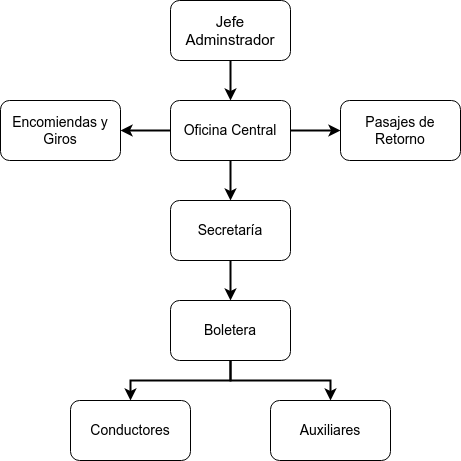
\includegraphics[width=0.55\textwidth]{imagenes/figura1_1.png} % Inserta una imagen
		
		\begin{flushleft}
			\hspace{1.20cm} \textbf{Nota.} Organigrama obtenido en entrevista con el administrador. % Nota al pie para esta figura
		\end{flushleft}
		\vspace{-16pt}
		\label{fig:figura1_1} % Etiqueta para referencia cruzada
	\end{figure}
	
	En la figura \ref{fig:figura1_1}, se observa la estructura organizativa de la empresa, destacando los diferentes cargos que desempeñan los empleados, que van desde el administrador hasta los auxiliares de apoyo. Dentro del negocio, se encuentran los boleteros y conductores, quienes son responsables de la atención directa a los pasajeros y la operación de los vehículos. Paralelamente, en la oficina central se gestionan las encomiendas, que son recibidas, clasificadas y preparadas para su envío. Cada uno de estos roles desempeña una función esencial para el funcionamiento eficiente y efectivo de la empresa, asegurando que tanto el transporte de pasajeros como la gestión de encomiendas se realicen con éxito y dentro de los estándares de calidad establecidos.
	
	\subsection*{Misión de la empresa}
	
	Proporcionar servicios de transporte y logística de alta calidad, enfocándose en la venta de pasajes y el envío de encomiendas, con el objetivo de satisfacer plenamente las necesidades de nuestros clientes. Nos comprometemos a ofrecer un servicio eficiente, seguro y confiable, contribuyendo al bienestar y comodidad de nuestros usuarios.
	
	\subsection*{Visión de la empresa}
	
	Ser la empresa líder en el sector del transporte y la logística en Bolivia, reconocida por nuestra innovación, eficiencia operativa y excelencia en el servicio al cliente. Aspiramos a expandir nuestra presencia y mejorar continuamente nuestros servicios para mantenernos a la vanguardia de la industria.
	
	\subsection*{Objetivo general de la empresa}
	El objetivo general de Cali Internacional es consolidar y expandir nuestra posición en el mercado del transporte y la logística, mejorando continuamente la calidad de nuestros servicios y adoptando tecnologías avanzadas para optimizar nuestras operaciones y satisfacer las necesidades cambiantes de nuestros clientes.
	
	\subsection*{Objetivos específicos de la empresa}
	
	\begin{itemize}[label=$\bullet$, left=0cm, labelsep = 1.05cm, topsep = 0pt, parsep = 0pt]
		
		\item Mejorar la experiencia del cliente mediante la oferta de servicios más rápidos, seguros y fiables.
		
		\item Capacitar continuamente a nuestro personal para asegurar que estén equipados con las habilidades necesarias para manejar las nuevas tecnologías y brindar un servicio de alta calidad.
		
		\item Implementar prácticas sostenibles en nuestras operaciones, minimizando el impacto ambiental y promoviendo la responsabilidad social corporativa.
		
	\end{itemize}	
	
	\subsection{Proyectos similares}
	
	Para la presente investigación se han considerado los siguientes antecedentes:
	
	\textcite{hurtado2019aplicacion}. ``Aplicación web administrativa para reserva de servicios de transporte y envío de encomiendas para la empresa Romero y Asociados (AMBASEUR) de la ciudad de Ambato''. En este proyecto, se implementó una aplicación web para automatizar los procesos manuales de una empresa, mejorando la gestión de reservas de transporte y envíos de encomiendas. La plataforma permite publicitar las actividades de la empresa y recopilar información precisa sobre los clientes. Desarrollada utilizando la metodología XP, la aplicación facilita la adaptación rápida a cambios y la incorporación de funciones adicionales, como un chat en línea, optimizando así la eficiencia y aumentando la base de clientes.
	
	\textcite{mora2022sistema}. ``Sistema gestión de servicio de viajes para la empresa Nuestra Señora de la Asunción C.I.S.A.'', esta investigación se centra en automatizar los procesos manuales de la empresa Nuestra Señora de la Asunción CISA mediante un sistema informático. En la primera etapa, se diagnosticaron los módulos de viajes, tráfico y ventas, entrevistando a responsables clave y recopilando los requerimientos necesarios. En la segunda etapa, se desarrolló un sistema informático web responsive que procesa automáticamente la información de estos módulos, integrando análisis, diseño y programación orientada a objetos, culminando en un sistema integrado con soporte audiovisual.
	
	\textcite{arevalo2021desarrollo}. ``Desarrollo de una aplicación web para
	agilizar los procesos de la compra y venta de boletos de buses interprovinciales en el terminal de Milagro.'', este proyecto desarrolló un sistema web para la compra y venta de boletos en el terminal terrestre del Cantón Milagro, con el objetivo de agilizar el proceso de boletería sin necesidad de contacto físico en ventanilla. Tras entrevistar a los socios del terminal para identificar los requisitos funcionales y no funcionales, se eligió la metodología ágil SCRUM para la organización y monitoreo constante del proyecto. El sistema se implementó utilizando Python, con Pycharm como IDE, Bootstrap 4 y Adminlte3 como plantillas, y PostgreSQL como base de datos. El resultado fue un sistema que satisface las necesidades del cliente, mejorando significativamente la experiencia de compra de boletos..
	
	\textcite{sosa2019sistema}. ``Sistema informático web para la gestión de pasajes de la empresa de transporte Turismo Transol Barranca S.A.C.'', en la tesis se propone como objetivo principal desarrollar un sistema informático web para la gestión de pasajes en la empresa de transportes Turismo Transol Barranca S.A.C., abarcando tanto la venta como la reserva de boletos. Este sistema busca optimizar el tiempo de procesamiento mediante el uso de tecnología web. La investigación se llevó a cabo con un enfoque descriptivo, un diseño no experimental y un corte transversal, utilizando una población de 42 personas y una muestra de 6 usuarios. Se aplicó la metodología Proceso Unificado de Rational (RUP), empleando el Lenguaje de Modelamiento Unificado (UML) para la construcción de diagramas de casos de uso, facilitando el análisis del software. El sistema fue desarrollado en Java, con MySQL como gestor de datos y MySQL Workbench 6.3 CE para el modelado de la base de datos, entre otras herramientas que ayudaron a cumplir los requisitos de diseño. Los resultados permitieron agilizar los procesos de venta y reserva de pasajes, mejorando el manejo de la información y extendiendo el alcance a los clientes, lo que fortaleció el posicionamiento competitivo de la empresa a nivel regional.
	
	\textcite{vivas2019propuesta}. ``Propuesta de implementación del sistema web de venta de boletos de viaje y gestión de encomiendas para la empresa Transportes Montero S.A.C. Piura; 2018.'', en esta investigación que fue desarrollada por la Escuela Profesional de Ingeniería de Sistemas de la Universidad Católica Los Ángeles de Chimbote, se centró en la mejora de procesos en organizaciones peruanas mediante la implementación de un sistema web para la venta de boletos y gestión de encomiendas en la empresa TRANSPORTES MONTERO S.A.C. en 2018. La investigación, de tipo cuantitativo y descriptivo con diseño no experimental y corte transversal, incluyó una muestra de 14 trabajadores. Los resultados mostraron que el 63 por ciento de los empleados consideraba que la empresa brindaba calidad en procesos y servicios, el 84 por ciento creía que los sistemas web agilizan los procesos, y el 81 por ciento opinaba que dichos sistemas eran eficientes, confirmando así la hipótesis planteada.
	
\section{OBJETO DE ESTUDIO}

	Software de logística y gestión de buses para transporte de pasajeros y envío de encomiendas, el cual va automatizar y mejorar la venta de pasajes, así como en la recepción, procesamiento y envío de encomiendas.
	
\section{PLANTEAMIENTO DEL PROBLEMA}

	La empresa de transportes Cali Internacional, se encuentra ante diversos retos importantes en cuanto a administrar sus procesos tanto de venta de pasajes como de envío de paquetería, estas operaciones son llevadas a cabo de forma manual, lo que genera ineficiencias en el funcionamiento, largos tiempos de espera para los clientes y una alta posibilidad de comoter errores. Además de afectar negativamente la experiencia del cliente, estos problemas también restringen las posibilidades de crecimiento y competencia efectiva en un mercado cada vez más digital, la implementación de soluciones tecnológicas integrales se ha convertido en una estrategia clave para optimizar procesos.  
	
	Algunos de los problemas mas frecuentes son:
	
	\begin{itemize}[label=$\bullet$, left=1.25cm, labelsep = 0.75cm, topsep = 0pt, parsep = 0pt]
		\item Largos tiempos de espera en la compra de pasajes y envío de encomiendas debido a la falta de automatización.
		\item Errores en la gestión de reservas y envíos, lo que puede resultar en pérdidas financieras y descontento entre los clientes.
		\item Falta de visibilidad y control sobre la demanda de servicios, lo que limita la capacidad de la empresa para ajustar su oferta y optimizar recursos.
		\item Dificultad para generar reportes y análisis que ayuden en la toma de decisiones estratégicas para la empresa.    
	\end{itemize}
	
	Por lo tanto, se plantea la siguiente interrogante:
	
	?`Cómo mejorar la venta de pasajes y la gestión de envío de encomiendas en la empresa Cali Internacional?
	
\section{JUSTIFICACIÓN}

	La implementación de un software de logística y gestión de buses para transporte de pasajeros y envío de encomiendas representa una respuesta estratégica ante la creciente demanda de soluciones tecnológicas en el sector de transporte y logística. La automatización de estos procesos no solo optimiza las operaciones internas, sino que también reduce significativamente los errores humanos y mejora la eficiencia. En vista de ello la mayoría de organizaciones se ha visto obligada a desarrollar un sistema web de calidad que brinde un mejor servicio a la comunidad, mejorando su imagen corporativa, demostrando que están al día con las nuevas tecnologías \parencite{nunez2005diseno}.
	
	Además, este proyecto aborda la necesidad de ofrecer un servicio más accesible y conveniente para los clientes. En un entorno donde la digitalización se ha vuelto imprescindible, la adopción de un sistema informático para estos servicios es una ventaja competitiva que no se puede ignorar.
	
	La digitalización de estos procesos en una plataforma única no solo agilizará las operaciones al automatizar tareas repetitivas y reducir la necesidad de intervención manual, sino que también mejorará significativamente la precisión y la transparencia de la información. Esta mejora permitirá a la empresa ofrecer un servicio más coherente y eficiente, ya que todos los datos estarán centralizados y accesibles en tiempo real, lo que facilitará una gestión más efectiva de los recursos. Además, la integración de estos procesos en una sola plataforma reducirá costos operativos al eliminar redundancias y optimizar el uso de la infraestructura tecnológica. En última instancia, esto resultará en una mejor experiencia para el cliente, aumentando su satisfacción al recibir un servicio más rápido y confiable, y posicionando a la empresa como líder en innovación y eficiencia dentro de su sector.
	
	Este proyecto se adapta a la necesidad de mantenerse al día con las tendencias tecnológicas actuales. Las empresas están siendo revolucionadas por la transformación digital, y aquellas que no se adapten corren el riesgo de quedarse atrás. Cuando la empresa implementa un software especializado, no solo se adapta a estas tendencias, sino que también está preparada para hacer frente a los desafíos futuros como la necesidad de incorporar nuevas tecnologías y responder a las demandas del mercado en constante cambio.
	
\section{OBJETIVOS}
	\subsection{Objetivo general}
	
		Desarrollar un software de logística y gestión de buses para transporte de pasajeros y envío de encomiendas para la empresa de transportes Cali Internacional de la ciudad de La Paz.
		
	\subsection{Objetivos específicos}
	
		\begin{itemize}[label=$\bullet$, left=0cm, labelsep = 1.05cm, topsep = 0pt, parsep = 0pt]
			
			\item Analizar los procesos actuales de venta de pasajes y envío de encomiendas en la empresa de transportes Cali Internacional para identificar las áreas de mejora y las necesidades tecnológicas específicas.
			\item Formular un diseño de interfaz centrado en la experiencia del usuario, facilitando su interacción con el sistema.
			\item Elaborar el diseño de la base de datos relacional a partir del análisis de los requerimientos del sistema, para llevar a la Tercera Forma Normal (3FN) y almacenar los datos.
			\item Diseñar el back-end para gestionar la venta de pasajes y el envío de encomiendas, asegurando la integración eficiente con la base de datos y la correcta ejecución de las operaciones solicitadas por los usuarios a través de la plataforma digital.    
			\item Generar reportes y análisis de datos que facilite la toma de decisiones informadas por parte de la administración de la empresa.
			
		\end{itemize}
		
\section{ALCANCES Y LÍMITES}
	\subsection{Alcances}
		
		El desarrollo de la presente investigación se encuentra dentro de los siguientes alcances:
		
		\begin{itemize}[label=$\bullet$, left=0cm, labelsep = 1.05cm, topsep = 0pt, parsep = 0pt]
			
			\item El proyecto abarcará la creación de una plataforma digital que permita a los usuarios realizar la compra de pasajes y la gestión de envíos de encomiendas de manera eficiente y segura.
			
			\item Se desarrollará un sistema de gestión de usuarios que permitirá a los empleados: iniciar sesión y gestionar las ventas de pasajes y envíos de encomiendas, mientras que los administradores podrán supervisar y manejar las operaciones.
			
			\item Se implementarán módulos que automatizarán tareas repetitivas como la generación de recibos, el seguimiento de envíos y la asignación de asientos en los buses de transportes.
			
			\item El sistema incluirá un módulo de reportes que permitirá a los administradores generar informes detallados sobre las ventas, la ocupación de los transportes, y la gestión de encomiendas.
			
			\item La plataforma será accesible desde diferentes tipos de dispositivos, incluyendo computadoras, tabletas, y smartphones, garantizando una experiencia de usuario consistente y accesible.
			
		\end{itemize}
		
	\subsection{Límites}
	
		Los límites de la investigación son los siguientes:
		
		\begin{itemize}[label=$\bullet$, left=0cm, labelsep = 1.05cm, topsep = 0pt, parsep = 0pt]
			
			\item El sistema estará diseñado inicialmente para cubrir las operaciones de la Empresa de transportes Cali Internacional en su sede de la Terminal de Buses en La Paz.
			
			\item La integración se centrará en los sistemas internos existentes de la empresa. %dejando de lado conexiones con plataformas o sistemas externos.
			
			\item El software será compatible con las plataformas y dispositivos especificados. %sin incluir soporte para otros sistemas no contemplados inicialmente.
			
			\item El soporte se limitará a las funcionalidades implementadas, las actualizaciones o desarrollos adicionales quedarán para fases futuras.
			
		\end{itemize}
		
\section{IMPORTANCIA DEL ESTUDIO}

	La importancia del estudio del proyecto radica en la necesidad de modernizar los procesos operativos de empresas de transporte y logística, especialmente en un entorno donde la eficiencia y la rapidez son factores clave para la competitividad. En la actualidad, muchas empresas en este sector aún dependen de sistemas manuales o desactualizados que ralentizan las operaciones, sino que también incrementan el riesgo de errores humanos, afectando directamente la calidad del servicio ofrecido al cliente. Este proyecto, por lo tanto, no solo aborda una necesidad tecnológica, sino que también busca mejorar la experiencia del cliente al ofrecerle un servicio más ágil y fiable.
	
	Desde una perspectiva social, este estudio tiene una importancia significativa al contribuir al avance tecnológico en un sector que afecta directamente a un gran número de personas. Al mejorar la eficiencia y la precisión en la venta de pasajes y el envío de encomiendas, se generan beneficios directos no solo para la empresa, sino también para los usuarios finales, quienes experimentarán un servicio más confiable y accesible. Esto, a su vez, puede fomentar una mayor confianza en los servicios digitales en general, impulsando el uso de la tecnología en otras áreas de la vida diaria.
	
	Finalmente, la importancia de este estudio también reside en su capacidad para servir como modelo para futuras implementaciones tecnológicas en empresas similares. La metodología empleada, así como los desafíos superados durante el desarrollo del software, pueden ofrecer valiosas lecciones para otros proyectos dentro del sector, promoviendo un enfoque más sistemático y eficiente en la adopción de tecnologías de la información en la industria del transporte y la logística.
	